\documentclass[12pt,a4paper,leqno]{report}
\usepackage[utf8]{inputenc}
\usepackage[czech,english]{babel}
\usepackage[T1]{fontenc}
\usepackage{amsmath}
\usepackage{amsfonts}
\usepackage{amssymb}
\usepackage{graphicx}
\usepackage{lmodern}
\usepackage{kpfonts}
\graphicspath{ {.} }
\usepackage[left=1.5cm,right=1.5cm,top=2cm,bottom=1.5cm]{geometry}
\author{Autor}
\title{Vyzařování fotovoltanického článku}
\begin{document}
\newpage
\tableofcontents
\newpage

\section{Úvod}

Cílem experimentu měření vyzařování fotovoltanického článku bylo zjistit homogenitu vyzařování při průchodu proudu článkem v propustném směru

\subsection{Popis měřícího zařízení}
\par Pro měření byl využit mikroskop *** se spektroskopem a digitálně řízeným XY stolem. Fotovoltanický článek by umístěn do speciálního kontaktovacího přípravku vytištěném na 3D tiskárně a umístěn na pohyblivý stůl mikroskopu. Sestava kontaktovacího přípravku a fotovoltanického článku je ukázána na Obr. ***. 

Fotovoltanický článek je k vodičům připojen pomocí pogo pinů, které jsou pozlacené a pro dobrý kontakt vybavené pružinou zajišťující dobrý kontakt mezi vodičem a vodivou vrstvou na článku.

\subsection{Fotovoltanický článek}
Pro měření byl vybrán fotovoltanický článek ***, který má vnější rozměry $80 \times 80 mm$. Ze spodní strany článku je nanesena vodivá vrstva, na kterou byly nakontaktovány přívodní vodiče. Aktivní plocha článku je $50\times50 mm$ a je rozdělena do jednotlivých "vodičů" tak, aby styčná obou polarit byla co největší.

\includegraphics[scale=1]{panel.eps}

\section{Měření}
\par Mikroskop byl nastaven do režimu skenování a integrace signálu z určitého roztahu vlnových délek ($1040.00 - 1060.00nm$).
\par Při měření článekem v propustném směru protékal proud $1A$ při napětí $21V$.

\subsection{Zpracování naměřených dat}
\par Z RAW dat ze záznamového SW mikroskopu byl pomocí python skriptu vytvořen .FITS soubor, který je lepší pro další analýzu naměřených dat. Do hlavičky soboru bylo vepsáno rozlišení na jednotlivých osách, takže ze snímku lze odpočítávat reálné rozměry.

\subsection{Celkový náhled}
\par Při prvním měření byla skenována celá aktivní plocha fotovoltanického článku v nižším rozlišení (4x0.25mm)

\begin{center}
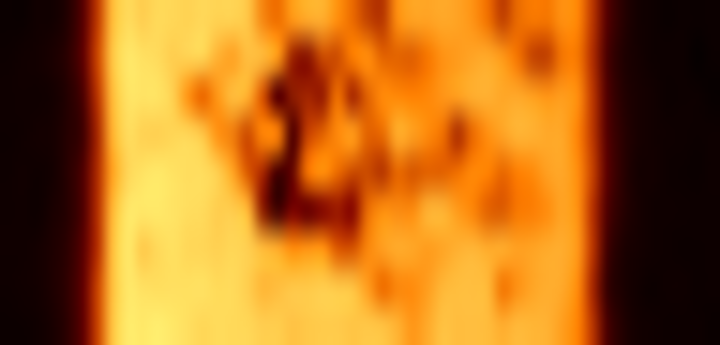
\includegraphics[width=15cm]{3e}
\end{center}

\subsection{Výběr č. 1}
První detailní výběr byl udělán v levém hodním rohu, kde vyzařování vypadá očekávané. Při detailním focení tohoto pole je vidět, že podél vodiče na spodní straně článku je intenzita záření větší. Toto zjasnění se opakuje s periodou $2.5 mm$.  

\begin{center}
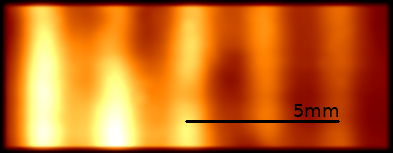
\includegraphics[width=15cm]{1}
\end{center}

\subsection{Výběr č. 2}
Druhý výběr byl vyfocen u středu článku, kde podle náhledu bylo vyzařování článku velmi nerovnoměrné.

\begin{center}
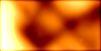
\includegraphics[width=15cm]{2}
\end{center}

\end{document}